\documentclass{llncs}
\usepackage{amsmath,amsfonts,wrapfig,graphicx,caption,url}
\usepackage{subcaption}
\usepackage[all]{xy}
\usepackage{tikz}
\usetikzlibrary{automata,positioning}
\captionsetup{compatibility=false}
\pagestyle{plain}

\newcommand{\Nat}{\mathbb{N}}
\newcommand{\Z}{\mathbb{Z}}
\newcommand{\st}{\mathsf{st}}
\newcommand{\str}{\mathsf{str}}
\newcommand{\encb}{\mathrm{eb}}
\newcommand{\EncB}{\mathrm{EM}}
\newcommand{\encm}{\mathrm{em}}
\newcommand{\CT}{\mathbb{CT}}
\newcommand{\dec}{\mathsf{dec}}
\newcommand{\enc}{\mathsf{enc}}


\begin{document}

\title{Verifiable Homomorphic Tallying for the Schulze Vote Counting
Scheme}

\author{Thomas Haines \inst{1} \and
      Dirk Pattinson\inst{2} \and Mukesh Tiwari \inst{2}}
\institute{Polyas GmbH, Germany \and
          Research School of Computer Science, ANU, Canberra}
\maketitle

\begin{abstract}
The encryption of ballots is crucial to maintaining integrity and 
anonymity in electronic voting schemes. It enables, amongst other 
things, each voter to verify that their encrypted ballot has been 
recorded as cast, by checking their ballot against a bulletin board. 

We present a verifiable homomorphic tallying scheme for the Schulze 
method that allows verification of the correctness of the count on the 
basis of encrypted ballots that only reveals the final tally. We 
achieve verifiability by using zero knowledge proofs for ballot 
validity and honest decryption of the final tally. Or formalisation 
takes places inside the Coq theorem prover and is based on an 
axiomatisation of cryptogtaphic primitives, and our main result is 
the correctness of homomorphic tallying. We then instantiate 
these primitives using an external library and show the feasibility 
of our approach by means of case studies.
\end{abstract}


\section{Introduction}

Secure elections are a balancing act between integrity and privacy:
achieving either is trivial but their combination is notoriously hard.
One of the key challenges faced by both paper based and electronic
elections is that results must substantiated with
verifiable evidence of their correctness while retaining the secrecy
of the individual ballot \cite{Bernhard:2017:PES}.  Technically, the
notion of ``verifiable evidence'' is captured by the term 
\emph{end-to-end (E2E) verifiability}, that is
\begin{itemize}
  \item every voter can verify that their ballot was cast as
  intended
  \item every voter can verify that their ballot was collected as
  cast
  \item everyone can verify final result on the basis of the
  collected ballots.
\end{itemize}
While end-to-end verifiability addresses the basic assumption that
no entity (software, hardware and participants) are inherently
trustworthy, ballot secrecy addresses the privacy problem.
Unfortunately, it appears as if coercion resistance is not achievable  
in the remote setting without relying on overly optimistic---to say the least---assumptions.
A weaker property called receipt-freeness captures the idea that an honest 
voter---while able to verify that their ballot was counted---is required to keep 
no information that a possible coercer could use to verifying how that voter had voted.

End to end verifiability and the related notation of software independence~\cite{Rivest:2008:PTRS}
 have been claimed properties for many voting schemes.  Kusters et al~\cite{Kusters:2010:CCS} gave
 a cryptographic formulation whose value is highlighted by the attacks it revealed in established voting 
 schemes~\cite{Kusters:2012:SP}.

The combination of privacy and integr, can be realised using cryptographic techniques, where
encrypted ballots (that the voters themselves cannot decrypt) are
published on a bulletin board, and the votes are then processed, and
the correctness of the final tally is substantiated, using
homomorphic encryption \cite{Hirt:2000:ERF} and verifiable shuffling
\cite{Bayer:2012:EZK}. (Separate techniques exist to prevent ballot
box stuffing and to guarantee cast-as-intended.)
Integrity can then be guaranteed by means of Zero Knowledge Proofs
(ZKP),
first studied by Goldwasser, Micali, and Rackoff~\cite{Goldwasser:1985:STOC}.
Informally, a ZKP is a probabilistic and interactive proof where one
entity provides eveidence about knowledge of a secret without
providing no information other than the truth of the statement, with
overwhelming probability. 
Later results~\cite{Goldreich:1991:ACM}\cite{Ben-Or:1988:CRYPTO} showed that 
all problems for which solutions can be efficiently verified have zero knowledge
proofs.


This paper addresses the problem of verifiable homomorphic tallying
for a preferential voting scheme, the Schulze voting scheme. We show
how the Schulze Method can be implemented in a theorem prover to
guarantee both provably correct and verifiable counting on the basis
of encrypted ballots, relative to an axiomatisation of the
cryptographic primitives. We then obtain, via program extraction, a
provably correct implementation of the vote counting, that we turn
into executable code by providing implementations of the primitives
based on a standard cryptographic library. We conclude by presenting
experimental results, and discuss trust the trust base, security and
privacy as well as the applicability of our work to real-world
scenarios. 

\subsection*{Leftover Text?}
In general, every election has purpose to elect candidates based on cast
  ballots while maintaining the integrity of election i.e. tallied correctly, 
  maintained individual ballot privacy, and coercions free. Many of these properties 
  we get for free in paper ballot election, but for electronic voting, not only 
  our protocol should have these properties, but at the same time they should be 
  evident. The inherent nature of tension (conflict) between privacy, keeping the votes 
  private and anonymous (unidentifiable), and universal verifiablity, anyone can verify
  tallying is correct (consistent) according to election rules, makes electronic 
  voting schemes very challenging. If we publish 
  the ballots in plain text it certainly offers universal verifiability, but at the same
  time it opens the possibility of coercion \cite{Benaloh:2009:SSC}, and if we don't
  publish then it certainly offers the more privacy, but hampers universal 
  verifiablity. \linebreak
      
  \smallskip\noindent\emph{The Schulze Method.} The Schulze Method
  \cite{Schulze:2011:NMC} is a preferential, single-winner vote
  counting scheme that is gaining popularity due to its relative
  simplicity while retaining near optimal fairness
  \cite{Rivest:2010:OSW}.  
  A \emph{ballot} is a rank-ordered list of
  candidates where different candidates may be given the same rank.
  The protocol proceeds in two steps, and first computes the
  \emph{margin matrix} $m$ where, for candidates $x$ and $y$, 
  \[ m(x, y) = \mbox{ballots that rank $x$ higher than $y$} - \mbox{ballots
  that rank $y$ higher than $x$}. \]
  We note that $m(x, y) = -m(y, x)$, i.e. the margin matrix is
  symmetric. In a second step, a \emph{generalised margin} $g$ is
  computed as the strongest path between two candidates
  \[ g(x,y) = \max \lbrace \str(p) \mid p \mbox{ path from $x$ to
  $y$} \rbrace \]
  where a path from $x$ to $y$ is simply a sequence $x = x_0, \dots,
  x_n = y$ of candidates, and the strength
  \[ \str(x_0, \dots, x_n) = \min \lbrace m(x_i, x_{i+1}) \mid i < n
  \rbrace  \]
  is the lowest margin encountered on a path.

  A candidate $w$ is a \emph{winner} if $g(w, x) \geq g(x, w)$ for
  all other candidates $x$. Informally, one may think of the
  generalised margin $g(x, y)$ as transitive accumulated support for
  $x$ over $y$, so that $x$ beats $y$ if $g(x,y) \geq g(y, x)$ and a
  winner is a candidate that cannot be beaten by anyone. Note that
  winners may not be uniquely determined (e.g. in the case where no
  ballots have been cast).

  In previous work \cite{Pattinson:2017:SVE} we have demonstrated
  how to achieve verifiability of counting plaintext ballots by
  producing a verifiable \emph{certificate} of the count. The
  certificate has two parts: The first part witnesses the
  computation of the margin function where each line of the
  certificate amounts to updating the margin function by a single
  ballot. The second part witnesses the determination of winners
  based on the margin function. In the first phase, i.e. the
  computation of the margin function, we perform the following
  operations for every ballot:
  \begin{enumerate}
    \item if the ballot is informal it will be discarded
    \item if the ballot is formal, the margin function will be
    updated
  \end{enumerate}
  The certificate then contains one line for each ballot and thus
  allows to independently verify the computation of the margin
  function. Based on the final margin function, the second part of
  the certificate presents verifiable evidence for the computation
  of winners. Specifically, if a candidate $w$ is a winner, it
  includes:
  \begin{enumerate}
    \item an integer $k$ and a path of strength $k$ from $w$ to any
    other candidate
    \item evidence, in the form of a co-closed set, of the fact that
    there cannot be a path of strength $> k$ from any other
    candidate to $w$.
  \end{enumerate}
  Crucially, the evidence of $w$ winning the election \emph{only}
  depends on the margin matrix. 
  We refer to \cite{Pattinson:2017:SVE} for details of the second
  part of the certificate as this will remain unchanged in the work
  we are reporting here.
    
  \smallskip\emph{Related Work.} 

\section{Verifiable Homomorphic Tallying}
\texttt{
  Bullet points of content for reference and later deletion
\begin{itemize}
  \item general protocol, comparision with plaintext counting
  \item two-phase structure: margin matrix, then winners with
  winners as before: encryption commutes with margin computation
  \item homomorphic computation of margin matrix, ballot
  representation
  \item computation of winners (as for plaintext)
\end{itemize}
}
The realisation of verifiable of homomorphic tallying that we are about to
describe follows the same two phases as the protocol: for each
ballot, we decide whether it is formal, and if so, homomorphically
update the margin function. We do this for every ballot, and record
this in the certificate. We then record the decryption of the margin
function in the certificate, and then publish the winner, together
with evidence based on the margin matrix, as in the case of counting
plaintext ballots (where evidence for winning also only depends on
the margin matrix).  We now describe the two phases in detail.

\smallskip\noindent\emph{Format of Ballots.} In preferential voting
schemes, ballots are rank-ordered lists of candidates. For the
Schulze Method, we require that all candidates are ranked, and two
candidates may be given the same rank. That is, a ballot is most
naturally represented as a function $b: C \to \Nat$ that assigns a
numerical rank to each candidate, and the computation of the margin
amounts to computing the sum
\[ m(x, y) = \sum_{b \in B} \begin{cases} +1 & b(x) > b(y) \\ 0 &
b(x) = b(y) \\ -1 & b(x) < b(y) \end{cases} \]
where $B$ is the multi-set of ballots, and each $b \in B$ is a
ranking function $b: C \to \Nat$ over a (finite) set $C$ of
candidates. 

We note that this representation of ballots is not well suited for
homomorphic computation of the margin matrix as practically feasible
homomorphic encryption schemes do not support comparison operators
and case distinctions as used in the formula above. 

We instead represent ballots as matrices
$b(x, y)$ where $b(x, y) = +1$ if $x$ is preferred
over $y$, $b(x, y) = -1$ if $y$ is preferred over $x$ and $b(x, y) =
0$ if $x$ and $y$ are equally preferred.

While the advantage of the first representation is that each ranking
function is necessarily a valid ranking, the advantage of the matrix 
representation is that the computation of
the margin matrix is simple, that is
\[ m(c, d) = \sum_{b \in B} b(x, y) \]
where $B$ is the multi-set of ballots (in matrix form), and can
moreover be transferred to the encrypted setting in a straight
forward way: if ballots are matrices $e(x,y)$ where $e(x,y)$ is the
encryption of an integer, then
\[ \encm = \bigoplus_{\encb \in \EncB} \encb(x, y) \]
where $\oplus$ denotes homomorphic addition, $\encb$ is an encrypted
ballot in matrix form (i.e. decrypting $\encb(x, y)$ indicates
whether $x$ is preferred over $y$), and $\EncB$ is the multi-set of
encrypted ballots. The disadvantage is that we need to verify that a
matrix ballot is indeed valid, that is
\begin{itemize}
\item that the decryption of $\encb(x, y)$ is indeed one of $1, 0$ or
$-1$
\item that $\encb$ indeed corresponds to a ranking function.
\end{itemize}

Indeed, to achieve verifiability, we not only need \emph{verify}
that a ballot is valid, we also need to \emph{evidence} its validity
(or otherwise) in the certificate.  

\smallskip\noindent\emph{Validity of Ballots.} By a plaintext
(matrix) ballot
we simply mean a function $b: C \times C \to \Z$,
where $C$ is the (finite) set of candidates. A 
plaintext ballot $b(x, y)$ 
is \emph{valid} if it is induced by a ranking function, i.e.
there exists a function $r: C \to \Nat$ such that $b(x, y) = 1$ if
$f(x) < f(y)$, $b(x, y) = 0$ if $f(x) = f(y)$ and $b(x, y) = -1$ if
$f(x) > f(y)$. A \emph{ciphertext (matrix) ballot} is a function
$\encb: C \times C \to \CT$ (where $\CT$ is a chosen set of
ciphertexts), and it is valid if the pointwise encryption, i.e. the
matrix ballot $b(x, y) = \dec(\enc(x,y))$ is valid (we use $\dec$ to
denote decryption). 

For a plaintext ballot, it is easy to decide whether it is
valid (and should be counted) or not (and should be discarded). We
use shuffles (ballot permutations) to evidence the validity of
encrypted ballots. One observes that a matrix ballot is valid if and
only if it is valid after permuting both rows and columns with the
same permutation. That is, $b(x,y)$ is valid if and only if $b'(x,y)$
is valid, where
\[ b'(x,y) = b(\pi(x), \pi(y)) \]
and $\pi: C \to C$ is a permutation of candidates. (Indeed, if $f$
is a ranking function for $b$, then $f \circ \pi$ is a ranking
function for $b'$). As a consequence, we can evidence the validity
of a ciphertext ballot $\encb$ by
\begin{itemize}
  \item publishing a shuffled version $\encb'$ of $\encb$, that is
  shuffled by a secret permutation, together with
  evidence that $\encb'$ is indeed a shuffle of $\encb$
  \item publishing the decryption $b'$ of $\encb'$ together with
  evidence that $b'$ is indeed the decryption of $\encb'$.
\end{itemize}

We use zero-knowledge proofs in the style of \cite{Bayer:2012:EZK}
to evidence the correctness of the shuffle, and zero-knowledge
proofs of honest decryption [reference missing] to evidence
correctness of decryption. This achieves ballot secrecy owing to the
fact that the permutation is never revealed.


In summary, the homomorphic computation of the margin matrix starts
with an encryption of the zero margin $\encm$, and for each
ciphertext ballot $\encb$
\begin{enumerate}
\item publishes a shuffle of $\encb$ together with a ZKP of 
correctness
\item publishes the decryption of a shuffle, together with a ZKP of
correctness
\item publishes the updated margin function, if the decrypted ballot
was valid, and
\item publishes the unchanged margin function, if the decrypted
ballot is not valid.
\end{enumerate}

\smallskip\noindent\emph{Witnessing of Winners.}
Once all ballots are counted, the computed margin is decrypted, and
winners (together with evidence of winning) are being computed as
for plaintext counting. We discuss this this part only briefly to be
self contained as it is as for plaintext counting
\cite{Pattinson:2017:SVE}. For each of the winners $w$ and each
candidate $c$ we publish
\begin{itemize}
\item a natural number $k(w, x)$
\item a path $w = x_0, \dots, x_n = x$ of strength $k$
\item a set $C(w, x)$ of pairs of candidates that is $k$-coclosed
and contains $(x, w)$
\end{itemize}
where a set $S$ is  $k$-coclosed if for all $(x,z) \in C$ we have
that $m(x, z) < k$ and either $m(x, y) < k$ or $(y,z) \in S$ for
all candidates $y$.  Informally, the first requirement ensures that
there is no direct path (of length one) between a pair $(x, z) \in
S$ ,and the second requirement ensures that for an element $(x, z)
\in S$, there cannot be a path that connects $x$ to an intermediate
node $y$ and then (transitively) to $z$ that is of strength $\geq
k$. 
We refer to \emph{op.cit.} for the (formal)
proofs of the fact that existence of co-closed sets witnesses the
winning conditions. 
  



\section{Realisation in a Theorem Prover}
\texttt{
  Bullet points of content for reference and later deletion
\begin{itemize}
  \item Axiomatisation of the cryptographic primitives
  \item correctness proof modulo correct crypto
  \item describe certificates and how to check them
  \item show that ``certificates certify''
\end{itemize}}
 Following from previous section, we now give elaborated view of formalization.
 The cryptographic primitives are treated as black box, and assumed 
each primitive holds certain properties which are modelled
 as axiom in Coq \cite{Bertot:2004:ITP}. We have total six axioms about 
 decryption, (secret) permutation, and shuffle, and we 
 invite the reader to examine the validity of these axioms, but for sake of 
 completeness and detail we sketch out the details of encryption scheme.
 
 The very first one among all these primitives 
are encryption function and decryption function with the trait, as suggested 
by name of axiom itself, that decryption is deterministic. 

\begin{verbatim}
  Inductive Group : Type :=
      group : Prime -> Generator -> Publickey -> Group. 

  Variable encrypt_message :
      Group -> plaintext -> ciphertext.
      
  Variable decrypt_message :
      Group -> Privatekey -> ciphertext -> plaintext.
 
  Axiom decryption_deterministic : forall (grp : Group) 
    (privatekey : Privatekey) (pt : plaintext), 
    decrypt_message grp privatekey (encrypt_message grp pt) = pt.
 \end{verbatim}
 
 Intuitively, it means that if we take some plaintext, encrypt it, and decrypt it 
 we should get the original plaintext. This axiom certainly forces us to decrypt
  the values 
 honestly during formalization, but to make sure that the certificate, which 
 will be discuss in a moment, can be checked 
 by scrutinizers to audit the election irrespective of how it was constructed, 
 we also produce the evidence in form of zero knowledge proof for honest decryption which
 can be verified later independently. In order to attain verifiability, 
 we need primitives to build 
 honest decryption zero knowledge proof to decouple the verification of election 
 outcome from code inspection used to produce result.
 As it is evident from the names itself, these primitives are about constructing honest
 decryption zero knowledge proof object, checking if a plaintext is indeed 
 honest decryption of claimed ciphertext using decryption zero knowledge proof object, 
 with property that what it means to be when honest decryption proof 
 checks out i.e. return true.
 
 \begin{verbatim}
   Variable construct_zero_knowledge_decryption_proof :
      Group -> Privatekey -> ciphertext -> DecZkp.

   Axiom verify_zero_knowledge_decryption_proof :
      Group -> plaintext -> ciphertext -> DecZkp -> bool. 
   
   Axiom verify_true :
      forall (grp : Group) (pt : plaintext) (ct : ciphertext) 
      (privatekey : Privatekey)
      (H : pt = decrypt_message grp privatekey ct),
      verify_zero_knowledge_decryption_proof grp pt ct
      (construct_zero_knowledge_decryption_proof grp privatekey ct) 
      = true.
 \end{verbatim}
 
 The axiom, \texttt{verify\_true}, itself states that if plaintext, \textit{pt}, 
 is honest
 decryption of ciphertext, \textit{ct}, then primitive
 \texttt{verify\_zero\_knowledge\_decryption\_proof} returns true for 
 suitably constructed zero knowledge proof.
 
 We have followed the similar line of 
 arguments for other cryptographic primitives used in formalization including generation
  of secret permutation, 
 the secret permutation is indeed a permutation, and ballots are indeed permuted by the
 claimed secret permutation by generating zero knowledge proof 
 for each operation performed during the counting ballots. Once we have axiomatized
  cryptographic primitives, we plug them into our 
 formalization to construct verifiable counting system. 
 
 At very high level, we can think of counting ballots as finite state machine or 
 automaton which has following states 
 \begin{itemize}
 \item starting state where all the ballots are uncounted, 
       no invalid ballot, and margin function is zero.
 \item intermediate steps where we inspect a ballot from list of uncounted ballots, 
 		and depending on its validity
       we either update the margin (if ballot is valid), or move to pile to 
       invalid ballots.
  \item final (accepting) state where no more uncounted ballots left, and use 
  		the computed margin to produce result  
 \end{itemize}
 
 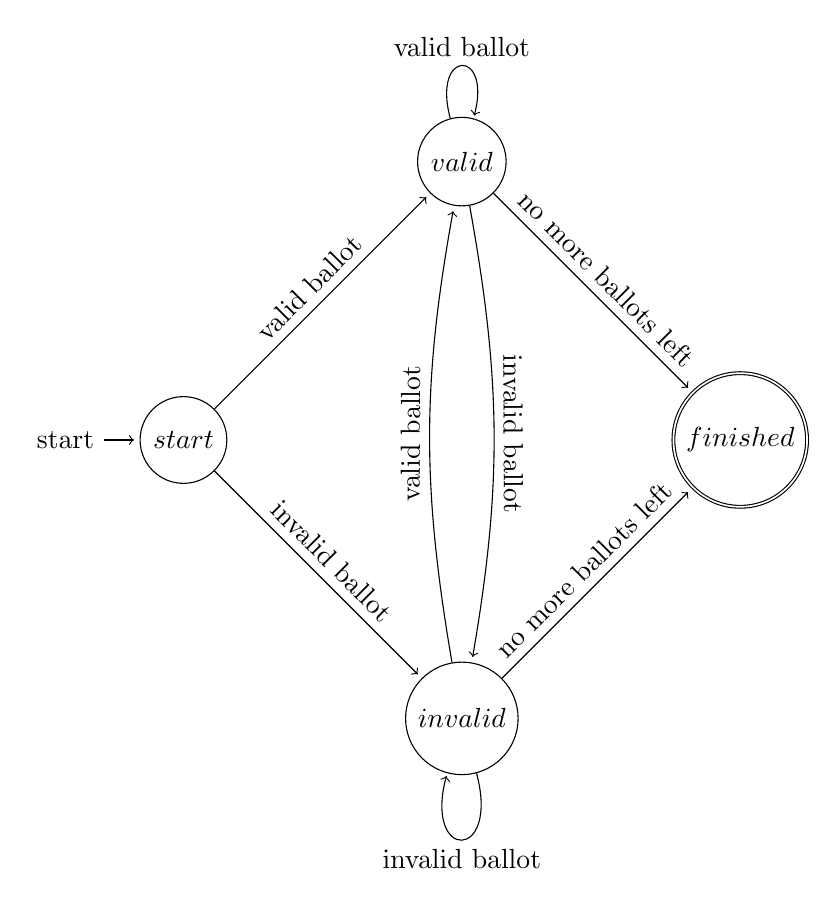
\begin{tikzpicture}[shorten >=2pt,node distance=5cm,on grid,auto] 
   \node[state,initial] (ecax)   {$start$}; 
   \node[state] (ecvalid) [above right=of ecax] {$valid$}; 
   \node[state] (ecinvalid) [below right=of ecax] {$invalid$}; 
   \node[state, accepting](ecdecrypt) [below right=of ecvalid] {$finished$};
    \path[->] 
    (ecax) edge  node [midway, above, sloped] {valid ballot} (ecvalid)
           edge  node  [above, sloped] {invalid ballot} (ecinvalid)
    (ecvalid) edge [bend left=10] node  [above, sloped] {invalid ballot} (ecinvalid)
    			edge  node [above, sloped,swap] {no more ballots left} (ecdecrypt) 
            edge [loop above] node {valid ballot} ()
    (ecinvalid) edge [bend left=10] node [above, sloped] {valid ballot} (ecvalid) 
    		   edge  node [above, sloped,swap] {no more ballots left} (ecdecrypt) 
           edge [loop below] node {invalid ballot} ();
\end{tikzpicture}



 We use Coq's dependent inductive data type facility to capture the notion of 
  finite state machine. To  be precise, the outcome
  of a election
 is inhabitant of inductive data type used to express the 
  different states of counting (finite state machine) using various constructors, 
  i.e. each constructor signifies some states of counting. Because of Coq's
  expressive (dependent) type system any arbitrary term can appear at type level, 
  we can  parameterised the counting (finite state machine) type by suitable 
  terms to  make sure that computation for constructing terms of type counting (finite 
  state machine) executes correctly.
 
  
 
 In order to capture the states of ballots and margin function during counting process, 
 we introduce inductive data type \textbf{EState}, and the interpretation of it is,  
  \begin{itemize}
  \item list of uncounted ballots which must be dealt with, 
  	and invalid ballots seen so far in counting process
  \item computed homomorphic margin so far
  \end{itemize}
  or decrypted margin function after all the ballots are counted, 
  or a boolean function used to determine the winner.
  
  
  
\begin{verbatim}
Inductive EState : Type :=
    | epartial : (list eballot * list eballot) ->
                 (cand -> cand -> ciphertext) -> EState
    | edecrypt : (cand -> cand -> plaintext) -> EState
    | ewinners : (cand -> bool) -> EState.
\end{verbatim}

We formalize the correct counting of homomorphic Schulze method by dependent inductive 
data type, \textbf{ECount}, which is parameterised by group, used for cryptographic 
primitive, list of cast ballots, and \textbf{EStates}. It is very crucial to 
notice that adding  \textbf{EState} as parameter to \textbf{ECount} forces the
 computation constructing the term of type \textbf{ECount} to follow the each step of protocol
  correctly. The computation expressed above follows 
  the same spirit as appending two dependent type 
  vector indexed over natural numbers of length n, and m would always 
  produce a vector of length  (n + m). Since Coq's expressive type system allows 
  us to represent this fact at type level only correct implementation of 
  append would type check.

 
 In order to show that protocol (counting)
 executed correctly, we need to show that it always ends up accepting state i.e. 
 produces the term (inhabitant) of type \textbf{ECount grp bs (ewinners w)}.



\begin{verbatim}
Inductive ECount (grp : Group) (bs : list eballot) : EState -> Type :=
 | ecax (us : list eballot) (encm : cand -> cand -> ciphertext)
        (decm : cand -> cand -> plaintext)
        (zkpdec : cand -> cand -> DecZkp) :
        us = bs ->
        (forall c d : cand, decm c d = 0) -> 
        (forall c d, verify_zero_knowledge_decryption_proof 
                  grp (decm c d) (encm c d) (zkpdec c d) = true) ->
        ECount grp bs (epartial (us, []) encm)
 | ecvalid (u : eballot) (v : eballot) (w : eballot)
           (b : pballot) (zkppermuv : cand -> ShuffleZkp)
           (zkppermvw : cand -> ShuffleZkp) 
           (zkpdecw : cand -> cand -> DecZkp)
           (cpi : Commitment) (zkpcpi : PermZkp)
           (us : list eballot) (m nm : cand -> cand -> ciphertext)
           (inbs : list eballot) :
   ECount grp bs (epartial (u :: us, inbs) m) ->
   matrix_ballot_valid b ->
   (verify_permutation_commitment grp (length cand_all) cpi zkpcpi = true) ->
   (forall c, verify_row_permutation_ballot grp u v cpi zkppermuv c = true) ->
   (forall c, verify_col_permutation_ballot grp v w cpi zkppermvw c = true) ->
   (forall c d, verify_zero_knowledge_decryption_proof 
                  grp (b c d) (w c d) (zkpdecw c d) = true) ->
   (forall c d, nm c d = homomorphic_addition grp (u c d) (m c d)) -> 
   ECount grp bs (epartial (us, inbs) nm)
 | ecinvalid (u : eballot) (v : eballot) (w : eballot)
             (b : pballot) (zkppermuv : cand -> ShuffleZkp)
             (zkppermvw : cand -> ShuffleZkp) 
             (zkpdecw : cand -> cand -> DecZkp)
             (cpi : Commitment) (zkpcpi : PermZkp)
             (us : list eballot) (m : cand -> cand -> ciphertext)
             (inbs : list eballot) :
   ECount grp bs (epartial (u :: us, inbs) m) ->
   ~matrix_ballot_valid b ->
   (verify_permutation_commitment grp (length cand_all) cpi zkpcpi = true) ->
   (forall c, verify_row_permutation_ballot grp u v cpi zkppermuv c = true) ->
   (forall c, verify_col_permutation_ballot grp v w cpi zkppermvw c = true) ->
   (forall c d, verify_zero_knowledge_decryption_proof 
                  grp (b c d) (w c d) (zkpdecw c d) = true) ->
   ECount grp bs (epartial (us, (u :: inbs)) m)
 | ecdecrypt inbs (encm : cand -> cand -> ciphertext)
             (decm : cand -> cand -> plaintext)
             (zkp : cand -> cand -> DecZkp) :
   ECount grp bs (epartial ([], inbs) encm) ->
   (forall c d, verify_zero_knowledge_decryption_proof
                  grp (decm c d) (encm c d) (zkp c d) = true) ->
   ECount grp bs (edecrypt decm)
 | ecfin dm w (d : (forall c, (wins_type dm c) + (loses_type dm c))) :
        ECount grp bs (edecrypt dm) ->
        (forall c, w c = true <-> (exists x, d c = inl x)) ->
        (forall c, w c = false <-> (exists x, d c = inr x)) ->
        ECount grp bs (ewinners w). 
\end{verbatim}
 

\begin{itemize}
\item The first constructor, \textbf{ecax}, marks the beginning the counting process by 
	  taking list of uncounted ballots, \textbf{us},
      encrypted margin function, \textbf{encm}, decrypted margin function, \textbf{decm}, 
      and zero knowledge proof, \textbf{zkpdec}, with proof that uncounted 
      ballots, \textbf{us}, are same as 
      cast ballots, \textbf{bs}, every entry in decrypted margin is 0, and 
      \textbf{decm} is indeed the 
      honest decryption of \textbf{encm} as honest decryption proof checker returns true.
 \item The constructor, \textbf{cvalid}, takes ballot \textbf{u} from uncounted 
 		ballots, ballot 
 		\textbf{v} which is row permutation of \textbf{u }by secret permutation, 
 		\textbf{w} which is column permutation of \textbf{v} by same secret permutation, 
 		\textbf{b} which is decryption of \text{w}, zero knowledge proof, 
 		\textbf{zkppermuv}, of v is indeed row permutation of u, 
 		zero knowledge proof, \textbf{zkppermvw}, of w is column permutation of 
 		v, zero knowledge proof, \textbf{zkpdecw}, of b is honest decryption w,
 		commitment, \textbf{cpi}, to secret permutation, and zero knowledge proof, 
 		\textbf{zkpcpi}, that we indeed committed to secret permutation 
 		with list of uncounted ballot, \textbf{us}, current margin, \textbf{m}, 
 		updated margin, \textbf{nm}, after adding ballot u homomorphically to 
 		current margin, \textbf{m}, and list of invalid ballots, \textbf{inbs}, 
 		seen so far with the usual proofs about validity data embedded in constructor. 
 \item The constructor, \textbf{cinvalid}, is very similar to \textbf{cvalid} except 
       rather than updating the running margin function, \textbf{m}, we move the ballot 
       to list of invalid ballot, \textbf{inbs}.
 \item The constructor, \textbf{ecdecrypt}, marks the finish of counting all the 
       ballot as it can be seen by state, 
       \textbf{ ECount grp bs (epartial ([], inbs) encm)}, with list of 
       invalid ballots, \textbf{inbs}, final encrypted margin, \textbf{encm}, 
       decrypted margin, \textbf{decm}, zero knowledge proof of honest 
       decryption, \textbf{zkp} with usual proofs about the consistency of data 
       in constructor. 
 \item The final constructor, \textbf{ecfin}, takes decrypted margin, \textbf{dm}, 
       boolean function, \textbf{w}, and d that delivers type level evidence of 
       winning and losing for each candidate.
   
\end{itemize}

We formally state that for every list of ballots, we can find a boolean function 
that decides winners, but what more important is that the term 
of type \textbf{ECount grp bs (ewinners f)} captures each step of 
execution which can be produced as evidence, known as certificate, 
to scrutineers for inspection.

\begin{verbatim}
Lemma pschulze_winners (grp : Group) (bs : list eballot) :
        existsT (f : cand -> bool), ECount grp bs (ewinners f).
\end{verbatim}

Coq extraction mechanism\cite{Letouzey:2003:NEC} allows us to extract its proofs into
programs retaining all the terms which lives in Type universe, and erases every term 
from Prop universe. After extracting Coq proofs into OCaml\cite{Leroy:2013:ORM} program, and plugging the 
cryptographic primitives into Unicrypt library via a thin wrapper written in 
OCaml using the library which calls Java function from OCaml (more details in next
section), and executing it on 
set of ballots produces the following certificate (as promised earlier), but 
the numbers appearing are very large and snipped because of space constraint.



\begin{verbatim}
M: AA(13.., 10..) AB(90.., 14..) AC(11.., 23..) BA(16.., 13..) BB(79.., 46..)
BC(12.., 14..) CA(50.., 53..) CB(70.., 68..) CC(23.., 82..), 
Decrypted margin [AA: 0 AB: 0 AC: 0 BA: 0 BB: 0 BC: 0 CA: 0 CB: 0 CC: 0], 
Zero Knowledge Proof of Honest Decryption: [..]
---------------------------------------------------------------------------
V: [AA(42.., 15..) AB(63.., 32..) AC(70, 44..) BA(47.., 34..) BB(16.., 28..)
BC(39.., 16..) CA(19.., 13..) CB(57.., 12..) CC(19.., 89..),..], I:  [], 
M: AA(12.., 11..) AB(13.., 66..) AC(16.., 14.) BA(48.., 31..) BB(15.., 52..)
BC(15.., 68..) CA(39.., 69..) CB(12.., 78..) CC(10.., 40..),
Row Permuted Ballot: AA(53.., 16..) AB(23.., 44..) AC(72.., 47..)
BA(10.., 19..) BB(74.., 16..) BC(20.., 60..) CA(44.., 10..) CB(12.., 16..)
CC(59.., 98..),
Column Permuted Ballot: AA(81.., 41..) AB(17.., 14..) AC(10.., 14..) 
BA(37.., 12..) BB(14.., 66..) BC(10.., 13..) CA(12.., 13..) 
CB(14.., 16..) CC(12.., 10..),
Decryption of Permuted Ballot: AA0 AB-1 AC1 BA1 BB0 BC1 CA-1 CB-1 CC0,
Zero Knowledge Proof of Row Permutation: [Tuple[...]], 
Zero Knowledge Proof of Column Permutation: [Tuple[..]], 
Zero Knowledge Proof of Decryption: [Triple[..]], 
Permutation commitment: Triple[..]
Zero Knowledge Proof of commitment: Tuple[..]
------------------------------------------------------------------------------------------
.
.
.
------------------------------------------------------------------------------------------
V: [AA(36.., 10..) AB(20.., 13..) AC(75.., 43..) BA(13.., 31..) BB(27.., 82..)
BC(31.., 50..) CA(16.., 11..) CB(74.., 15..) CC(26.., 36..)], I: [], M: AA(86.., 38..)
AB(21.., 14..) AC(16.., 25..) BA(16.., 22..) BB(18.., 15..) BC(11.., 63..)
CA(15.., 34..) CB(76.., 18..) CC(11.., 10..), 
Row Permuted Ballot: .., Column Permuted Ballot: .., 
Decryption of Permuted Ballot: AA0 AB-10 AC1 BA10 BB0 BC1 CA-1 CB-1 CC0,
Zero Knowledge Proof of Row Permutation: [..],
Zero Knowledge Proof of Column Permutation: [..], 
Zero Knowledge Proof of Decryption: [..], 
Permutation commitment: Triple[..], 
Zero Knowledge Proof of commitment: Tuple[..]
------------------------------------------------------------------------------------
V: [], I: [AA(36.., 10..) AB(20.., 13..) AC(75.., 43..) BA(13.., 31..) BB(27.., 82..)
BC(31.., 50..) CA(16.., 11..) CB(74.., 15..) CC(26.., 36..)], M: .., 
DM: [AA: 0 AB: 4 AC: 4 BA: -4 BB: 0 BC: 4 CA: -4 CB: -4 CC: 0],
Zero Knowledge Proof of Decryption: [..]
--------------------------------------------------------------------------------------------------------------------------------------------------------------------------------------------------------------------------------------------------------------------------------------------------------------------------------------------------------------------------------------------------------------------------------------------------------------------------------------------------------------------------------------------------------------------------------------------------------------------------------------------------------------------------------------------------------------------------------------------------------------------------------------------------------------------------------------------------------------------------------------------------------------------------------------------------------------------------------------------------------------------------------------------------------------------------------------------------------------------------------------------------------------------------------------------------------------------------------------------------------------------------------------------------------------------------------------------------------------------------------------------------------------------------------------------------------------------------------------------------------------------------------------------------------------------------------------------------------------------------------------------------------------------------------------------------------------------------------------------------------------------------------------------------------------------------------------------------------------------------------------------------------------------------------------------------------------------------------------------------------------------------------------------------------------------------------------------------------------------------------------------------------------------------------------------------------------------------------------------------------------------------------------------------------------------------------------------------------------------------------------------------------------------
DM: [AA: 0 AB: 4 AC: 4 BA: -4 BB: 0 BC: 4 CA: -4 CB: -4 CC: 0]
winning: A
   for B: path A --> B of strenght 4, 5-coclosed set: [(B,A),(C,A),(C,B)]
   for C: path A --> C of strenght 4, 5-coclosed set: [(B,A),(C,A),(C,B)] 
losing: B
   exists A: path A --> B of strength 4, 4-coclosed set: [(A,A),(B,A),(B,B),(C,A),
   (C,B),(C,C)]
losing: C
   exists A: path A --> C of strength 4, 4-coclosed set: [(A,A),(B,A),(B,B),
   (C,A),(C,B),(C,C)]

\end{verbatim}

We have 3 candidates A, B, and C. In the beginning of computation, we publish 
the information embedded in constructor \textbf{ecax} i.e.  
encrypted zero margin, M, its decryption to show that all the 
entries are 0, and zero knowledge proof of honest decryption. 
In next line, we display the 
first ballot from uncounted pile, V, that we are about to count, 
pile of invalid ballots so far, I, 
running encrypted margin, M, row permutation, i.e. permuting each row by secret
 permutation, of ballot that we are counting, 
column permutation, i.e. permuting each column by same secret permutation, 
 of ballot obtained from previous step after row permutation,
decryption of final permuted ballot with zero knowledge proof of each operation. 
Depending on the validity of finally permuted ballot, either we update the 
margin function homomorphically, \textbf{cvalid}, 
or move it to pile of invalid ballots, \textbf{cinvalid}. We continue 
until every ballot is counted. Once counting is finished then we decrypt the fully 
constructed margin function with zero knowledge, \textbf{ecdecrypt}. 
In final step, we show the evidence provided by 
constructor \textbf{ecfin}, which included decrypted margin, winners(loser) with
evidence about winning(losing).


Not only we provide certificate to verify the computation, but we provide 
proof of correctness against fully verified implementation of 
Schulze method \cite{Pattinson:2017:SVE} assuming 
that if there one to one correspondence between plaintext ballots and encrypted ballots,
i.e. if plaintext ballot is valid then its encryption is also valid and if 
encrypted ballot is valid then it's decryption is also valid, 
then computing winners via plaintext ballot is same as encrypted ballot and vice-versa. 
\begin{verbatim}
  Lemma final_correctness :
    forall  (grp : Group) (bs : list ballot) (pbs : list pballot) 
    (ebs : list eballot) (w : cand -> bool)
    (H : pbs = map (fun x => 
         (fun c d => decrypt_message grp privatekey (x c d))) ebs)
    (H2 : mapping_ballot_pballot bs pbs), 
    Count bs (winners w) -> ECount grp ebs (ewinners w).
      
  Lemma final_correctness_rev :
    forall  (grp : Group) (bs : list ballot) (pbs : list pballot) 
    (ebs : list eballot) (w : cand -> bool)
    (H : pbs = map (fun x => 
         (fun c d => decrypt_message grp privatekey (x c d))) ebs)
    (H2 : mapping_ballot_pballot bs pbs),
    ECount grp ebs (ewinners w) -> Count bs (winners w).
\end{verbatim}







\section{Extraction and Experiments}
\begin{itemize}
  \item extension of Unicrypt with homomorphic addition
  \item coupling between library and extracted code
  \item need for light weight wrappers
  \item experimental results: how long, how much memory, certicicate
  size
\end{itemize}

\section{Analysis}

\noindent\emph{Summary.} The main contribution of our formalisation is that of independently
verifiable \emph{evidence} for a set of candidates to be the winners
of an election counted according to the Schulze method. Our main
claim is that that our notion of evidence is both safeguarding the
privacy of the individual ballot (as the count is based on encrypted
ballots) and is verifiable at the same time (by means of zero
knowledge proofs). To do this, we have axiomatised a set of
cryptographic primitives to deal with encryption, decryption,
correctness of shuffles and correctness of decryption. From formal
and constructive proof of the fact that such evidence can always be
obtained, we have then extracted executable code that is provably
correct by construction and produces election winners together with
evidence once implementations for the cryptographic primitives are
supplied.

In a second step, we have supplied an implementation of these
primitives, largely based on the Unicrypt Library. Our expertiments
have demonstrated that this approach is feasible, but quite clearly
much work is still needed to improve efficiency. 

\smallskip\noindent\emph{Assumptions for Provable Correctness.}
While we claim that the end product embodies a high level of
reliability, our approach necessarily leaves some gaps between the
executable and the formal proofs. First and foremost, this is of
course the implementation of the cryptographic primitives in an
external (and unverified) library. We have minimised this gap by
basing our implementation on a purpose-specific existing library
(Unicrypt) to which we relegate most of the functionality. Another
gap is the extraction mechanism of the Coq theorem prover which does
not come with formal correctness guarantees that reach down to the
machine code level such as for example CakeML~\cite{Kumar:2014:CVI}.

\smallskip\noindent\emph{Modelling Assumptions.} In our modelling of
the cryptographic primitives, in particular the zero knowledge
proofs, we have assumed that zero knowledge proofs can be verified,
whereas in reality zero-knowledge proofs just confirm facts with
very high probability which we have deliberately  ignored. As a
consequence our correctness assertions only hold to the level
of probability that is guaranteed by zero knowledge proofs.

\smallskip\noindent\emph{Scalability.} We have analysed the
feasibility of the extracted code by counting an increasing number
of ballots. While this demonstrates a proof of concept, our results
show that the cryptographic layer adds significant overhead compared
to plaintext tallying \cite{Pattinson:2017:SVE}.  Our present
hypothesis is that this overhead is created by the various layers of
bindings between the executable (extracted into OCaml) and the
Unicrypt library (implemented in Java) as each appears to be very
efficient individually. 

\smallskip\noindent\emph{Future Work.} Our axiomatisation of the
needed cryptographic primitives lays the foundation of creating a
verified library. For scalability, a more detailed analysis (and
profiling) of the software artefact are necessary. Orthogonal to
what we have presented here, it would also be of interest to develop
a provably correct verifier for the notion of certificate presented
here. 

\bibliographystyle{plain}
\bibliography{all2,delta2}

\appendix
\section*{Notes and Leftovers Start Here}



\section{Format of Ballots}

%\begin{itemize}
%  \item motivate the choice of ballots and compare with plaintext
%  version
%  \item define encryption function that changes representation
%  \item a ballot is valid if and only if there is evidence that
%  proves its validity
%  \item encrypting valid ballots leads to valid ballots, and the
%  same for invalid ballots 
%  \item 
  Each ballot, B, is a $n\times$n matrix where n is the number of candidates 
  participating in
  election. Each voter marks the entry (i,j) in ballot B as 1 if he prefers 
  candidate i over j
  otherwise mark it 0. No candidate is preferred over itself, so all the 
  diagonal entries are 
  filled with 0. 
  The reason for representing a ballot as a matrix because the precise 
\begin{itemize}
  \item motivate the choice of ballots and compare with plaintext
  version
  \item define encryption function that changes representation
  \item a ballot is valid if and only if there is evidence that
  proves its validity
  \item encrypting valid ballots leads to valid ballots, and the
  same for invalid ballots 
  
  \item Each ballot, B, is a $n\times$n matrix where n is the number of 
  candidates participating in election. Each voter marks the entry (i, j) as 1 
  and (j, i) as -1 in ballot B if  he prefers candidate $i$ over $j$. If the voter 
  has no preference between candidate $i$ and $j $ i.e. they are ranked 
  same then voter would mark entry (i, j) and (j, i) as 0. No candidate is 
  preferred over itself, so all the diagonal entries are  filled with 0.  The
   reason for representing a ballot as a matrix because the precise 

  nature of our algorithm involving no decryption of individual ballot to protect
  ballot privacy,  facilitating the scrutiny for validity, and ease of computing 
  cumulative margin over encrypted data to compute the winners. 
  
  
   

  Each entry in ballot is encrypted by additive ElGamal i.e. encrypting the 
  message m as ($g^{r}, h^{r}g^{m}$) where $g$ is generator of cycle group $G$, and 
  $h = g^{x}$ is private key. After performing the encryption, a plain text ballot 
  i.e. matrix having entries of 0, and 1 changes to a matrix having pair for 

  \item  Each entry in ballot is encrypted by additive ElGamal i.e. encrypting the 
  message m as ($g^{r}, h^{r}g^{m}$) where $g$ is generator of cycle group $G$ of order $q$,  private key $x$ and randomness $r$  are randomly  
  chosen from \{1, \ldots, $q$ - 1\}, and public key is computed as 
  $h = g^{x}$. It is important to note that generator $g$, private key $x$ and 
  public key $h$ are generated during key generation phase of Elgamal 
  algorithm while  randomness $r$  is generated fresh for each message.
 \end{itemize} 
  After performing the encryption, a plain text ballot 
  i.e. matrix having entries of -1,  0, and 1 changes to a matrix having pair for 
  each entry representing the encryption of corresponding plain text. 
  A representation of plain text ballot  
  \[  
  \begin{bmatrix}
    x_{11}       & x_{12} & x_{13} & \dots & x_{1n} \\
    x_{21}       & x_{22} & x_{23} & \dots & x_{2n} \\
    \hdotsfor{5} \\
    x_{n1}       & x_{n2} & x_{n3} & \dots & x_{nn}
  \end{bmatrix}\] and data structure used to represent this ballot in 
  Coq is
  \begin{verbatim}
   Definition plaintext := Z.
   Definition pballot := cand -> cand -> plaintext.
  \end{verbatim}
  A representation of encrypted ballot 
  \[  
  \begin{bmatrix}
    (y_{11}, z_{11}) & (y_{12}, z_{12}) & (y_{13}, z_{13}) & \dots & (y_{1n}, z_{1n}) \\
    (y_{21}, z_{21}) & (y_{22}, z_{22}) & (y_{23}, z_{23}) & \dots & (y_{2n}, z_{2n}) \\
    \hdotsfor{5} \\
    (y_{n1}, z_{n1}) & (y_{n2}, z_{n2}) & (y_{n3}, z_{n3}) & \dots & (y_{nn}, z_{nn})
  \end{bmatrix}\] and the corresponding data structure in Coq is 
  \begin{verbatim}
   Definition ciphertext := (Z * Z)%type.
   Definition eballot := cand -> cand -> ciphertext.
  \end{verbatim}
     
 The reason for using additive ElGamal is that it's composability on ciphertext 
 under same public key. In short,  (Should I explain the algorithm here that 
  why this scheme works or explain it encryption section ?)
 \begin{center}  
	$enc_{k}(m_{1}) * enc_{k}(m_{2}) = enc_{k} (m_{1} + m_{2})$
 \end{center}
 Our choice of representing ballot as matrix comes with price. A malicious 
 voter could try to encode all sort of ballots including cyclic ones i.e. candidate
 $A$ is preferred over candidate $B$, candidate $B$ is preferred over candidate $C$, 
 and candidate $C$ is preferred over candidate $A$, and it is clear that voter has
 not expressed his choices clearly as it can not be expressed in linear preference order 
 and should not be considered for counting, or 
 he could inflate his favourite candidate by any other number higher that 1, and It 
 makes the ballot invalid because any value greater that 1 in a ballot would be similar
 to voter has casted more than one vote. We define a ballot is valid if all the 
 entries in matrix is encryption of -1, 0 and 1, and there is no cycle in it. Formally, We have
 \begin{verbatim}
 
	Definition matrix_ballot_valid (p : pballot) :=
      (forall c d : cand, In (p c d) [-1; 0; 1]) /\
	       valid cand p.  
 
 
 Definition valid (A : Type) (P : A -> A -> Z) :=
      exists f : A -> nat,
          forall c d : A,
          (P c d = 1 <-> (f c < f d)%nat) /\
          (P c d = 0 <-> f c = f d) /\ 
          (P c d = -1 <-> (f c > f d)%nat)
          
     (* Which one should keep ? Upper one is in Code while this one is 
        more intutive after expanding the definition *) 
    Definition matrix_ballot_valid (p : pballot) :=
      (forall c d : cand, In (p c d) [-1; 0; 1]) /\
      (exists f : A -> nat,
          forall c d : A,
          (p c d = 1 <-> (f c < f d)%nat) /\
          (p c d = 0 <-> f c = f d) /\ 
          (p c d = -1 <-> (f c > f d)%nat))
    
 \end{verbatim}
 Intuitively, it says that a ballot p is valid if we can find a function which
  expresses 
 the notion of linear preference ordering for all candidates, and 
 we prove that we can decide for each ballot if it is valid or not 
 \begin{verbatim}
  Lemma matrix_ballot_valid_dec : 
        forall p : pballot, {matrix_ballot_valid p} +
                            {~matrix_ballot_valid p}.
 \end{verbatim}
 
 By now, a attentive reader would note that we have claimed that we don't decrypt
 the ballot to preserve the privacy, so how can we decide the validity 
 without decrypting the original ballot. We will discuss our whole cryptographic 
 scheme in next section, but to quench the thrust of reader for now, we have 
 proved that if ballot p was valid
 before encryption, then encrypting it followed by permuting each row by 
 secret permutation $\sigma$ and permuting again the each column of resulting matrix 
 from  previous step by same permutation, $\sigma$, and decrypting it back would
 still 
 lead to valid ballot. 
 (* Write this same Lemma for $matrix_ballot_valid$ then 
      any permutation of it is valid and if it is invalid then any permutation of 
       it is invalid. The proof is already lying there in other proofs so 
       it's basically copy paste.   *)
 \begin{verbatim}
 Lemma perm_presv_validity :
     forall (A : Type) (P : A -> A -> Z),
       (forall c d : A, {c = d} + {c <> d}) ->
       (forall c d : A, {P c d = 1} + {P c d = 0} + {P c d = -1}) ->
       forall sig : A -> A, Bijective sig -> valid A P <-> valid A (perm A P sig)
 \end{verbatim}
 And similarly, for invalid ballot 
 \begin{verbatim}
 Lemma not_perm_persv_validity :
  forall (A : Type) (P : A -> A -> Z),
       (forall c d : A, {c = d} + {c <> d}) ->
       (forall c d : A, {P c d = 1} + {P c d = 0} + {P c d = -1}) ->
       forall sig : A -> A, Bijective sig -> ~ valid A P <-> ~ valid A (perm A P sig).
\end{verbatim}
%\end{itemize}

\section{Homomorphic Computation of Margin}
\begin{itemize}
  \item motivate and introduce how the margin is computed
  homomorphcially
  \item prove that encrption commutes with computation of margin
  
\end{itemize}

\section{Homomorphic Counting}
\begin{itemize}
  \item prove that encruption commutes with computation of winners
  \item discuss the evidence: publish cleartext margin function
  \item describe certificates and how to check them
\end{itemize}

\section{Experimental Results}
\begin{itemize}
  \item how long does it take, and how much memory?
  \item how large are the certificates?
\end{itemize}


\section{Discussion and Further Work}



One aspect that we have not considered here is encryption of
ballots to safe-guard voter privacy which can be incorporated using
protocols such as shuffle-sum \cite{Benaloh:2009:SSC} and
homomorphic encryption \cite{Yi:2014:HEA}. The key idea here is to
formalise a given voting scheme based on encrypted ballots, and then
to establish a homomorphic property: the decryption of the result
obtained from encrypted ballots is the same as the result obtained from
the decrypted ballots.  We leave this to further work.

%\bibliographystyle{myplain}
%\bibliography{all2,delta2}


\end{document}
